\ProvidesFile{Mvc.tex}[Model View Controller]


\subsection{Model View Controller (MVC)}
\label{section::MVC}

В этом разделе наша задача обсудить один из важных паттернов используемых для GUI -- MVC паттерн.

\subsubsection{Что происходит}

Если мы хотим написать интерактивное приложение, то полезно писать код так, чтобы ядро приложения и графические библиотеки были отделены друг от друга.
Если вам нужно внести изменение в пользовательский интерфейс, ядро приложения не должно никак от этого пострадать.
Если вы вносите изменения в ядро, которое не нарушает контракт соединения с графической библиотекой, то это не должно ломать ваш код.
Для того чтобы обеспечить такое поведение принято выделять 3 основные компоненты.
\begin{enumerate}
\item Model.
Это внутреннее представление данных.
Данный объект содержит все состояние.

\item View.
Графическое представление данных.
Этот объект использует данные модели и отображает их пользователю.

\item Controller.
Объект, управляющей моделью, на основе сигналов от пользователя.
\end{enumerate}
Важно понимать, что это не значит, что вся программа содержит одну модель, одну view и один контроллер.
Подобное разделение на роли может происходить на более мелком уровне.

\paragraph{Пример}

Предположим, что у вас есть простейшее приложение состоящее из окна и поля для введения и редактирования текста.
В этом случае у нас есть следующие три компонента:
\[
\xymatrix{
  {
  \boxed{
  \begin{tabular}{c}
  \textbf{Model}\\
    string:\;"1f"\\
    int:\;1
  \end{tabular}
  }
  }
  &{}
  &{
  \parbox{3cm}{\centering\textbf{View}\\ 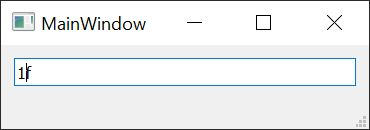
\includegraphics[scale=0.5]{Figures/edit4.jpg}}
  }
  \\
  {}
  &{
  \boxed{
    \textbf{Controller}
  }
  }
  &{}
}
\]
Обратите внимание, что модель в этом случае не просто строка, а строка и позиция курсора.
Потому что окно для редактирования умеет показывать положение курсора для редактирования.
Логически данные (или состояние) хранится только в модели.
View ничего не хранит (логически не хранит, всякое кэширование данных и прочие вспомогательные структуры могут использоваться).
Важно, что только данные из модели являются настоящей правдой.
То есть без модели View не знает что рисовать.
У нее нет дефолтного состояния.
Контроллер -- это просто кусок кода, который принимает команды от пользователя и на основе них вызывает методы у модели.

\paragraph{Виды соединений}

Теперь когда у нас есть три компоненты надо понять как они друг с другом связаны.
Бывают два типа соединения:
\begin{center}
\begin{tabular}{cc}
{
$
\xymatrix{
  {\phantom{\text{Model}}}
  {\save
  [].[dd]*+[F--]\frm{}
  \restore
  } 
  &{\text{View1}}\\
  {\text{Model}}\ar@{-->}[ru]\ar@{-->}[r]\ar@{-->}[rd]&{\text{View2}}\\
  {}&{\text{View3}}\\
}
$
}
&
{
$
\xymatrix{
  {\text{Controller1}}\ar@{->>}[rd]&  {\phantom{\text{Model}}}
  {\save
  [].[dd]*+[F--]\frm{}
  \restore
  }
  \\
  {\text{Controller2}}\ar@{->>}[r]&{\text{Model}}\\
  {\text{Controller3}}\ar@{->>}[ru]&{}\\
}
$
}\vspace{0.5cm}\\
{
$
\xymatrix{
  {\text{Observable}}\ar@{-->}[r]&{\text{Observer}}
}
$
}
&
{
$
\xymatrix{
  {\text{Controller}}\ar@{->>}[r]&{\text{Model}}
}
$
}
\end{tabular}
\end{center}
Соединение представленное слева -- это push уведомления, которые представляют из себя Observalbe/Observer соединения, которое обсуждалось в разделе~\ref{section::Observer}.
Его главная особенность в том, что у нас один источник данных и много слушателей для этих данных.
Соединение справа -- это соединение Host/Handle, которое обсуждалось в разделе~\ref{section::TrackingPtr}.
Его основная особенность, что наоборот может быть много контроллеров на одну модель.

\subsubsection{Модель для MVC}

\paragraph{Обычная модель}

Обычно принято рисовать такую общую картинку для описания того, как соединяются компоненты между собой.
\[
\xymatrix{
  {\phantom{\text{Model}}}
  {\save
  [].[dd]*+[F--]\frm{}
  \restore
  }  
  &{\text{View}}\ar@{-->}[dd]\\
  {\text{Model}}\ar@{-->}[ru]&{}\\
  {}&{\text{Controller}}\ar@{->>}[lu]\\
}
\]
Пунктиром тут обозначены границы ядра программы.
Эта часть вообще не зависит ни от каких графических библиотек.
Эта часть даже не знает, что она является частью интерактивного приложения.
\begin{itemize}
\item
Модель внутри ядра -- основной источник данных.
Как только View присоединилась к Model, то Model тут же отправляет ей свое текущее состояние и View тут же его отрисовывает таким, какое оно есть.
Если у модели что-то поменялось, то она тут же оповещает свою View (или несколько View), чтобы та отобразила ее в текущем состоянии.
К одной модели может быть подсоединено много разных View.
Вы можете пытаться отображать данные в разных форматах в разных окнах или вообще принципиально разных способом.

\item
Контроллер же наоборот управляет моделью по указателю.
Точнее, чтобы соединение было надежным это надо делать через handle.
В данном случае Model является host.
А внутри контроллера содержится handle для управления моделью.
У одной модели может быть много контроллеров.
Например, один контроллер от клавиатуры, а другой от GUI.
Потому тут не подходит Observable/Observer соединение.

\item
И последняя часть -- соединение между View и Controller.
Обычно представляют, что это тоже push уведомления по типу Observer/Observable.
Почему это так.
Ну потому что если пользователь нажал на кнопку экрана, то это возникло какое-то действие, о котором знает View.
И значит она должна сообщить теперь об этом Controller.
Однако так бывает не всегда.
Бывает что источник сигнала не внутри View.
Например ввод с клавиатуры.
\end{itemize}
Когда вы пишите свое интерактивное приложение, вы вряд ли пишите все GUI и Message Driven System-у с нуля сами, вы скорее всего используете готовые решения.
А тогда есть подозрения, что ни одна из библиотек не поддерживает возможности соединяться по Observable/Observer соединению, в особенности используемому вами в вашем проекте.
Потому полезно эту концептуальную картину немного представить в другом виде.

\paragraph{Другая модель}

Вот еще чуть более реалистичная картинка.
\[
\xymatrix{
  {\phantom{\text{Model}}}
  {\save
  [].[dd]*+[F--]\frm{}
  \restore
  }  
  &{\text{View}}\ar[r]&{\text{GUI}}
  {\save
  [].[dd]*+[F--]\frm{}
  \restore
  }\\
  {\text{Model}}\ar@{-->}[ru]&{}&{\text{Library}}\\
  {}&{\text{Controller}}\ar@{->>}[lu]&{\text{Message System}}\ar@{~>}[l]\\
}
\]
Здесь виды соединений:
\[
\xymatrix@R=5pt@C=15pt{
  {\text{Observable}(1)}\ar@{-->}[r]&{\text{Observer}(n)}&  {\text{View}(1)}\ar@{->}[r]&{\text{GUI}(1)}\\
  {\text{Controller}(n)}\ar@{->>}[r]&{\text{Model}(1)}&  {\text{Message System}(1)}\ar@{~>}[r]&{\text{Controller}(n)}\\
}
\]
Давайте прокомментируем соединения.
\begin{enumerate}
\item Model$\to$View -- как и раньше Observable/Observer соединение для поставления данных из модели во View.
Соединение от одной модели к многим View.

\item Controller$\to$Model -- как и раньше соединение по типу Host/Handle для управления моделью.
Соединение от нескольких контроллеров к одной модели.

\item View$\to$GUI.
Если вы используете готовую GUI библиотеку, то для каждого View объекта вы будете использовать библиотечный код для имплементации GUI.
Обычно для одной View вы создаете один объект, представляющей состояние View (состояние графического изображения для пользователя, но НЕ состояние модели).
Это обычно один в один соединение.

\item Message System$\to$Controller.
В интерактивных приложениях обычно используются Message Driven Systems, которые обсуждались в разделе~\ref{section::MDS}.
Любые действия пользователя тогда перерабатываются в сообщения системы.
А потому контроллер должен прослушивать данные сообщения и после этого совершать нужные действия с моделью.
Тут есть такая тонкость.
Все ли необходимые для совершения действия данные прилетают внутри сообщения.
Бывает так, что не все.
А тогда у контроллера должна быть возможность эти данные получить.
А это значит, что он может хранить какие-то указатели или лучше handle-ы на графические компоненты, где должны быть данные.
\end{enumerate}

\subsubsection{Демонстрация как работает MVC}

Давайте вернемся к первой модели в маленьком масштабе из предыдущего примера.
Напомню, что у нас есть простое окно с полем для ввода и изменения текста.
Предположим, что мы поставили курсор и нажали друг за другом клавиши <<1>>, <<f>> и <<$\leftarrow$>>.
Тогда видимое еоведение будет таким
\[
\xymatrix@R=40pt@C=50pt{
  {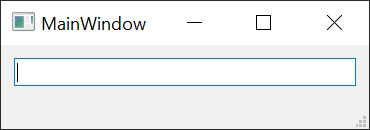
\includegraphics[scale=0.5]{Figures/edit1.jpg}}
  \ar@{|->}[r]^{\boxed{1}}
  &
  {{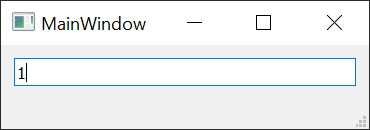
\includegraphics[scale=0.5]{Figures/edit2.jpg}}}
  \ar@{|->}[dl]+(-2,11)|{\boxed{f}}
  \\
  {{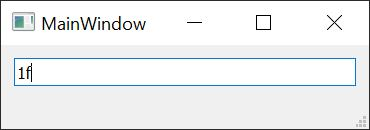
\includegraphics[scale=0.5]{Figures/edit3.jpg}}}
  \ar@{|->}[r]^{\boxed{\leftarrow}}
  &
  {{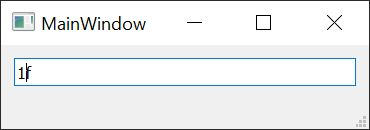
\includegraphics[scale=0.5]{Figures/edit4.jpg}}}
}
\]
Давайте посмотрим, как такая система должна работать по внутренней логике MVC паттерна.
У любой интерактивной программы есть две стадии:
\begin{enumerate}
\item Инициализация всех ресурсов для начала исполнения.

\item Исполнение программы.
\end{enumerate}
Во время первой стадии нам нужно проделать следующее:
\begin{enumerate}
\item Создать Model.

\item Создать View.

\item Создать Controller.

\item Соединить Model$\to$View.

\item Соединить View$\to$Controller.

\item Соединить Controller$\to$Model.
\end{enumerate}
Во время второй стадии собранная система реагирует на сообщения Message Driven System-ы.

Начнем с создания объектов.
В конструкторе нашего приложения мы создаем Model, View и Controller.
Логически будем представлять их так.
\[
\xymatrix{
  {
  \boxed{
  \begin{tabular}{c}
    string:\;""\\
    int:\;0
  \end{tabular}
  }
  }
  %\ar@{-->}[rr]
  &{}&
  {
  \parbox{3cm}{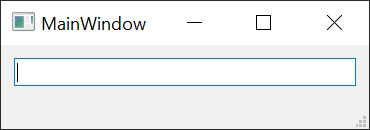
\includegraphics[scale=0.5]{Figures/edit1.jpg}}
  }
  %\ar@{-->}[dl]
  \\
  {}&
  {
  {\boxed{
    \text{Ctrl}
  }}
  }
  %\ar@{->>}[ul]
  &{}
}
\]
Обратите внимание, что сейчас у меня показывается окно с пустым полем для ввода и позицией коретки на нуле.
Однако, это не очень правильное представление.
По хорошему в этом состоянии View просто показывает белое поле без информации.
View лишь знает геометрию поля для ввода, но не его содержание.
И лишь в момент соединения Model и View, данные от модели поступают во View и она их отрисовывает.
\[
\xymatrix{
  {
  \boxed{
  \begin{tabular}{c}
    string:\;""\\
    int:\;0
  \end{tabular}
  }
  }
  \ar@{-->}[rr]^{\text{Оповещение}}
  &{}&
  {
  \parbox{3cm}{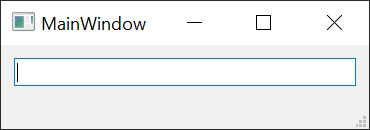
\includegraphics[scale=0.5]{Figures/edit1.jpg}}
  }
  %\ar@{-->}[dl]
  \\
  {}&
  {
  {\boxed{
    \text{Ctrl}
  }}
  }
  %\ar@{->>}[ul]
  &{}
}
\]
Полностью собранная схема будет выглядеть так
\[
\xymatrix{
  {
  \boxed{
  \begin{tabular}{c}
    string:\;""\\
    int:\;0
  \end{tabular}
  }
  }
  \ar@{-->}[rr]
  &{}&
  {
  \parbox{3cm}{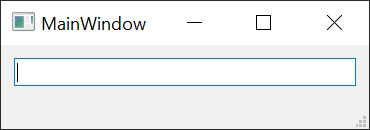
\includegraphics[scale=0.5]{Figures/edit1.jpg}}
  }
  \ar@{-->}[dl]
  \\
  {}&
  {
  \boxed{
    \text{Ctrl}
  }
  }
  \ar@{->>}[ul]
  &{}
}
\]
На этом закончилась стадия конструирования.
Перейдем к стадии обработки сообщений.
На этой стадии мы считаем, что пользователь последовательно выполнил следующие команды
\begin{enumerate}
\item Нажата клавиша <<1>>.

\item Нажата клавиша <<f>>.

\item Нажата клавиша <<$\leftarrow$>> (стрелка влево).
\end{enumerate}
Ниже показана поэтапная схема, отражающая, что происходит в MVC контуре.
Красным обозначается текущая в данный момент операция.
\begin{center}
\newcounter{listitem}
\newcommand{\listitem}{\par\addtocounter{listitem}{1}\noindent\textbf{\arabic{listitem})}\; }
\begin{longtable}{ll}
{
\listitem
\begin{minipage}[\baselineskip]{8cm}
\[
\xymatrix{
  {
  \boxed{
  \begin{tabular}{c}
    string:\;``''\\
    int:\;0
  \end{tabular}
  }
  }
  \ar@{-->}[rr]
  &{}
  &{
  \parbox{3cm}{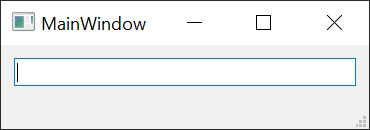
\includegraphics[scale=0.45]{Figures/edit1.jpg}}
  }
  \ar@{-->}@[red][dl]|-{\boxed{1}}
  \\
  {}
  &{
  \boxed{
    \text{Ctrl}
  }
  }
  \ar@{->>}[ul]
  &{}
}
\]
\end{minipage}
}&{
\listitem
\begin{minipage}[\baselineskip]{8cm}
\[
\xymatrix{
  {
  \boxed{
  \begin{tabular}{c}
    string:\;``''\\
    int:\;0
  \end{tabular}
  }
  }
  \ar@{-->}[rr]
  &{}
  &{
  \parbox{3cm}{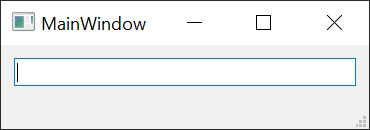
\includegraphics[scale=0.45]{Figures/edit1.jpg}}
  }
  \ar@{-->}[dl]
  \\
  {}
  &{
  \boxed{
    \text{Ctrl}
  }
  }
  \ar@{->>}@[red][ul]
  &{}
}
\]
\end{minipage}
}\\\hline
{
\listitem
\begin{minipage}[\baselineskip]{8cm}
\[
\xymatrix{
  {
  \boxed{
  \begin{tabular}{c}
    string:\;\color{red}{``1''}\\
    int:\;\color{red}{1}
  \end{tabular}
  }
  }
  \ar@{-->}[rr]
  &{}
  &{
  \parbox{3cm}{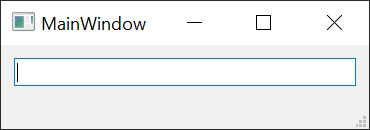
\includegraphics[scale=0.45]{Figures/edit1.jpg}}
  }
  \ar@{-->}[dl]
  \\
  {}
  &{
  \boxed{
    \text{Ctrl}
  }
  }
  \ar@{->>}[ul]
  &{}
}
\]
\end{minipage}
}&{
\listitem
\begin{minipage}[\baselineskip]{8cm}
\[
\xymatrix{
  {
  \boxed{
  \begin{tabular}{c}
    string:\;``1''\\
    int:\;1
  \end{tabular}
  }
  }
  \ar@{-->}@[red][rr]
  &{}
  &{
  \parbox{3cm}{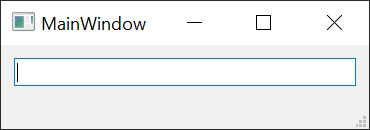
\includegraphics[scale=0.45]{Figures/edit1.jpg}}
  }
  \ar@{-->}[dl]
  \\
  {}
  &{
  \boxed{
    \text{Ctrl}
  }
  }
  \ar@{->>}[ul]
  &{}
}
\]
\end{minipage}
}\\\hline
{
\listitem
\begin{minipage}[\baselineskip]{8cm}
\[
\xymatrix{
  {
  \boxed{
  \begin{tabular}{c}
    string:\;``1''\\
    int:\;1
  \end{tabular}
  }
  }
  \ar@{-->}[rr]
  &{}
  &{
  \parbox{3cm}{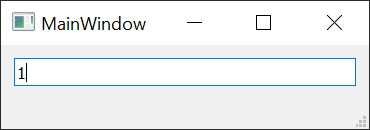
\includegraphics[scale=0.45]{Figures/edit2.jpg}}
  }
  \ar@{-->}[dl]
  \\
  {}
  &{
  \boxed{
    \text{Ctrl}
  }
  }
  \ar@{->>}[ul]
  &{}
}
\]
\end{minipage}
}&{
\listitem
\begin{minipage}[\baselineskip]{8cm}
\[
\xymatrix{
  {
  \boxed{
  \begin{tabular}{c}
    string:\;``1''\\
    int:\;1
  \end{tabular}
  }
  }
  \ar@{-->}[rr]
  &{}
  &{
  \parbox{3cm}{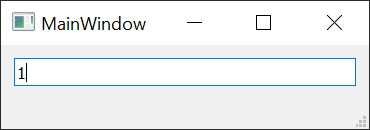
\includegraphics[scale=0.45]{Figures/edit2.jpg}}
  }
  \ar@{-->}@[red][dl]|-{\boxed{f}}
  \\
  {}
  &{
  \boxed{
    \text{Ctrl}
  }
  }
  \ar@{->>}[ul]
  &{}
}
\]
\end{minipage}
}\\\hline
{
\listitem
\begin{minipage}[\baselineskip]{8cm}
\[
\xymatrix{
  {
  \boxed{
  \begin{tabular}{c}
    string:\;``1''\\
    int:\;1
  \end{tabular}
  }
  }
  \ar@{-->}[rr]
  &{}
  &{
  \parbox{3cm}{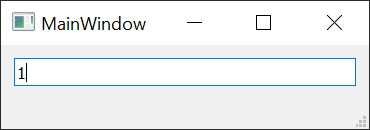
\includegraphics[scale=0.45]{Figures/edit2.jpg}}
  }
  \ar@{-->}[dl]
  \\
  {}
  &{
  \boxed{
    \text{Ctrl}
  }
  }
  \ar@{->>}@[red][ul]
  &{}
}
\]
\end{minipage}
}&{
\listitem
\begin{minipage}[\baselineskip]{8cm}
\[
\xymatrix{
  {
  \boxed{
  \begin{tabular}{c}
    string:\;\color{red}{``1f''}\\
    int:\;\color{red}{2}
  \end{tabular}
  }
  }
  \ar@{-->}[rr]
  &{}
  &{
  \parbox{3cm}{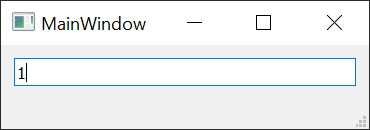
\includegraphics[scale=0.45]{Figures/edit2.jpg}}
  }
  \ar@{-->}[dl]
  \\
  {}
  &{
  \boxed{
    \text{Ctrl}
  }
  }
  \ar@{->>}[ul]
  &{}
}
\]
\end{minipage}
}\\\hline
{
\listitem
\begin{minipage}[\baselineskip]{8cm}
\[
\xymatrix{
  {
  \boxed{
  \begin{tabular}{c}
    string:\;``1f''\\
    int:\;2
  \end{tabular}
  }
  }
  \ar@{-->}@[red][rr]
  &{}
  &{
  \parbox{3cm}{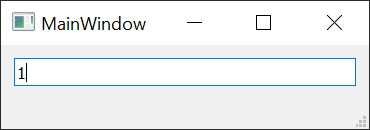
\includegraphics[scale=0.45]{Figures/edit2.jpg}}
  }
  \ar@{-->}[dl]
  \\
  {}
  &{
  \boxed{
    \text{Ctrl}
  }
  }
  \ar@{->>}[ul]
  &{}
}
\]
\end{minipage}
}&{
\listitem
\begin{minipage}[\baselineskip]{8cm}
\[
\xymatrix{
  {
  \boxed{
  \begin{tabular}{c}
    string:\;``1f''\\
    int:\;2
  \end{tabular}
  }
  }
  \ar@{-->}[rr]
  &{}
  &{
  \parbox{3cm}{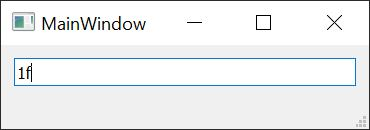
\includegraphics[scale=0.45]{Figures/edit3.jpg}}
  }
  \ar@{-->}[dl]
  \\
  {}
  &{
  \boxed{
    \text{Ctrl}
  }
  }
  \ar@{->>}[ul]
  &{}
}
\]
\end{minipage}
}\\\hline
{
\listitem
\begin{minipage}[\baselineskip]{8cm}
\[
\xymatrix{
  {
  \boxed{
  \begin{tabular}{c}
    string:\;``1f''\\
    int:\;2
  \end{tabular}
  }
  }
  \ar@{-->}[rr]
  &{}
  &{
  \parbox{3cm}{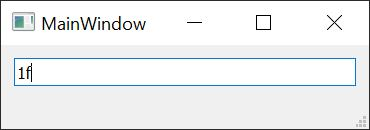
\includegraphics[scale=0.45]{Figures/edit3.jpg}}
  }
  \ar@{-->}@[red][dl]|-{\boxed{\leftarrow}}
  \\
  {}
  &{
  \boxed{
    \text{Ctrl}
  }
  }
  \ar@{->>}[ul]
  &{}
}
\]
\end{minipage}
}&{
\listitem
\begin{minipage}[\baselineskip]{8cm}
\[
\xymatrix{
  {
  \boxed{
  \begin{tabular}{c}
    string:\;``1f''\\
    int:\;2
  \end{tabular}
  }
  }
  \ar@{-->}[rr]
  &{}
  &{
  \parbox{3cm}{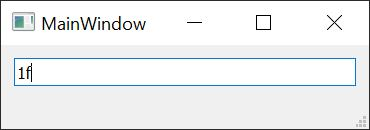
\includegraphics[scale=0.45]{Figures/edit3.jpg}}
  }
  \ar@{-->}[dl]
  \\
  {}
  &{
  \boxed{
    \text{Ctrl}
  }
  }
  \ar@{->>}@[red][ul]
  &{}
}
\]
\end{minipage}
}\\\hline
{
\listitem
\begin{minipage}[\baselineskip]{8cm}
\[
\xymatrix{
  {
  \boxed{
  \begin{tabular}{c}
    string:\;``1f''\\
    int:\;\color{red}{1}
  \end{tabular}
  }
  }
  \ar@{-->}[rr]
  &{}
  &{
  \parbox{3cm}{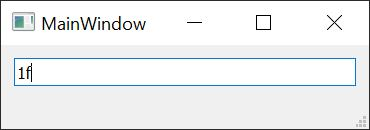
\includegraphics[scale=0.45]{Figures/edit3.jpg}}
  }
  \ar@{-->}[dl]
  \\
  {}
  &{
  \boxed{
    \text{Ctrl}
  }
  }
  \ar@{->>}[ul]
  &{}
}
\]
\end{minipage}
}&{
\listitem
\begin{minipage}[\baselineskip]{8cm}
\[
\xymatrix{
  {
  \boxed{
  \begin{tabular}{c}
    string:\;``1f''\\
    int:\;1
  \end{tabular}
  }
  }
  \ar@{-->}@[red][rr]
  &{}
  &{
  \parbox{3cm}{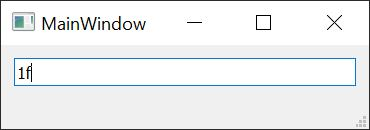
\includegraphics[scale=0.45]{Figures/edit3.jpg}}
  }
  \ar@{-->}[dl]
  \\
  {}
  &{
  \boxed{
    \text{Ctrl}
  }
  }
  \ar@{->>}[ul]
  &{}
}
\]
\end{minipage}
}\\\hline
{
\listitem
\begin{minipage}[\baselineskip]{8cm}
\[
\xymatrix{
  {
  \boxed{
  \begin{tabular}{c}
    string:\;``1f''\\
    int:\;1
  \end{tabular}
  }
  }
  \ar@{-->}[rr]
  &{}
  &{
  \parbox{3cm}{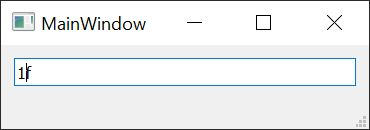
\includegraphics[scale=0.45]{Figures/edit4.jpg}}
  }
  \ar@{-->}[dl]
  \\
  {}
  &{
  \boxed{
    \text{Ctrl}
  }
  }
  \ar@{->>}[ul]
  &{}
}
\]
\end{minipage}
}&{
}\\
\end{longtable}
\end{center}
Давайте прокомментируем как это работает.
\begin{enumerate}
\item После нажатия на клавишу <<1>> оповещается соответствующий графический компонент, в нашем случае это поле для ввода текста.
В этот момент поле ввода для текста НЕ меняется, потому что у него нет внутреннего состояния, оно всегда отражает состояние модели.
Вместо этого этот компонент посылает сообщение контроллеру, что нажата клавиша <<1>>.

\item На этом этапе контроллер видит, что клавиша <<1>> дает символ ``1'', который надо поместить в строку внутри модели и сдвинуть коретку на $1$ вперед.

\item На этом слайде красным помечено изменение состояния модели.

\item Как только модель изменила свое состояние, она оповещает всех, кто на нее подписан, чтобы они пришли с ней в одно состояние.
В частности оповещается поле для ввода текста о новом состоянии модели.

\item И вот на этом шаге поле для ввода текста получив новое состояние модели отражает его в виде строки <<1>> и положения картки после цифры $1$.

\item После нажатия на клавишу <<f>>, оповещается графически элемент -- поле для ввода текста.
После чего это поле посылает сигнал контроллеру.

\item Контроллер видит, что эта клавиша дает символ.
И зовет метод модели, который добавляет этот символ в месте расположения каретки.

\item Здесь красным обозначено новое состояние модели.
Теперь хранится строка <<1f>> и новое положение каретки $2$.

\item Теперь модель оповещает текстовое поле о своем новом состоянии.

\item Текстовое поле отражает новое состояние модели.
То есть оно отображает строку <<1f>> и новое положение коретки в конце строки.

\item Теперь после нажатия пользователем клавишы <<$\leftarrow$>> -- стрелка влево, оповещается соответствующий графический компонент -- поле ввода для текста.
Этот компонент посылает сигнал контроллеру.

\item Контроллер видит, что это клавиша отвечает за навигацию по тексту и вызывает у модели метод сдвига коретки влево.

\item Новое положение коретки в модели отмечено красным.
Строка не меняется.

\item Теперь модель оповещает всех о своем новом состоянии.

\item И наконец-то текстовое поле отображает текущую строку <<1f>> и положение коретки между этих двух символов.
\end{enumerate}
Этот пример хорошо показывает общую логику работы MVC.
Все данные хранятся в модели, она единственный источник информации.
View всегда отражает только то, что ей прилетело от модели и логически не имеет своего состояния.
Контроллер же управляет моделью напрямую.

\paragraph{Замечание про Controller}

В такой схеме может показаться странным, что нам нужно использовать View и Controller как две разные сущности.
Потому что все равно все данные из View идут в Controller и потом по этим данным дергается модель.
Причина почему выделяется контроллер -- мы не хотим, чтобы в GUI коде была бизнес логика управления моделью.
Мы не хотим, чтобы GUI зависело от ядра.
Мы хотим, чтобы GUI зависило от данных, которые прилетают из ядра по Observer паттерну, но мы не хотим чтобы были какие-либо другие зависимости.
Чтобы отрезать GUI код от ядра и вводится контроллер.
В этом случае View лишь зависит от двух типов данных: получаемые от модели и отсылаемые контроллеру.
View не принимает никаких решений, не умеет управлять моделью, не содержит никакой логики.
Вся логика управления уходит в Controller.

\subsubsection{MVC и реальность}

Если вы работаете с готовыми графическими библиотеками, то к сожалению или к счастью, они не предоставляют stateless (без состояния) графических компонент (или не всегда их предоставляют).
А потому любой графический компонент или widget в реальной библиотеки сам из себя представляет уже готовый MVC контур запеченый в один объект.
И если вы пытаетесь использовать этот widget как View, у вас получится какая-то такая картинка:
\[
\xymatrix{
  {}&{}&{}&{\text{\textbf{Widget}}}&{}\\
  {}&{}&{\text{M}}\ar@{-->}[rr]
  {\save
  [].[rrd]*+[F-]\frm{}
  \restore
  }
  &{}&{\text{V}}\ar@{-->}[dl]\\
  {\text{Model}}\ar@{-->}@(u,l)[urr]&{}&{}\ar@{-->}@(d,r)[dl]&{\text{C}}\ar@{->>}[ul]&{}\\
  {}&{\text{Ctrl}}\ar@{->>}@(l,d)[ul]&{}&{}&{}\\
}
\]
В бокс справа на картинке объединены внутренности Widget.
При использовании View, которая имеет состояние, вы по сути имеете две модели, которые вам придется согласовывать.
А согласование двух моделей при двустороннем общении -- это всегда огромная проблема.
У вас возникают следующие проблемы
\begin{enumerate}
\item Двойное обновление модели.

\item Гашение обратной связи.
\end{enumerate}
Давайте промоделируем одно оповещение контроллера в схеме представленной выше.
Предположим на пользователь совершил какое-то действие, которое заставило View внутри Widget-а оповестить контроллер внутри Widget-а.
\begin{center}
\setcounter{listitem}{0}
\newcommand{\listitem}{\par\addtocounter{listitem}{1}\noindent\textbf{\arabic{listitem})}\; }
\begin{longtable}{ll}
{
\listitem
\begin{minipage}[\baselineskip]{8cm}
\[
\xymatrix@R=15pt@C=15pt{
  {}&{}&{}&{\textbf{Qt Widget}}&{}\\
  {}&{}&{\text{M}}\ar@{-->}[rr]
  {\save
  [].[rrd]*+[F-]\frm{}
  \restore
  }
  &{}&{\text{V}}\ar@{-->}@[red][dl]\\
  {\text{Model}}\ar@{-->}@(u,l)[urr]&{}&{}\ar@{-->}@(d,r)[dl]&{\text{C}}\ar@{->>}[ul]&{}\\
  {}&{\text{Ctrl}}\ar@{->>}@(l,d)[ul]&{}&{}&{}\\
}
\]
\end{minipage}
}&{
\listitem
\begin{minipage}[\baselineskip]{8cm}
\[
\xymatrix@R=15pt@C=15pt{
  {}&{}&{}&{\textbf{Qt Widget}}&{}\\
  {}&{}&{\text{M}}\ar@{-->}[rr]
  {\save
  [].[rrd]*+[F-]\frm{}
  \restore
  }
  &{}&{\text{V}}\ar@{-->}[dl]\\
  {\text{Model}}\ar@{-->}@(u,l)[urr]&{}&{}\ar@{-->}@(d,r)[dl]&{\text{C}}\ar@{->>}@[red][ul]&{}\\
  {}&{\text{Ctrl}}\ar@{->>}@(l,d)[ul]&{}&{}&{}\\
}
\]
\end{minipage}
}\\\hline
{
\listitem
\begin{minipage}[\baselineskip]{8cm}
\[
\xymatrix@R=15pt@C=15pt{
  {}&{}&{}&{\textbf{Qt Widget}}&{}\\
  {}&{}&{\text{M}}\ar@{-->}@[red][rr]
  {\save
  [].[rrd]*+[F-]\frm{}
  \restore
  }
  &{}&{\text{V}}\ar@{-->}[dl]\\
  {\text{Model}}\ar@{-->}@(u,l)[urr]&{}&{}\ar@{-->}@(d,r)[dl]&{\text{C}}\ar@{->>}[ul]&{}\\
  {}&{\text{Ctrl}}\ar@{->>}@(l,d)[ul]&{}&{}&{}\\
}
\]
\end{minipage}
}&{
\listitem
\begin{minipage}[\baselineskip]{8cm}
\[
\xymatrix@R=15pt@C=15pt{
  {}&{}&{}&{\textbf{Qt Widget}}&{}\\
  {}&{}&{\text{M}}\ar@{-->}[rr]
  {\save
  [].[rrd]*+[F-]\frm{}
  \restore
  }
  &{}&{\text{V}}\ar@{-->}[dl]\\
  {\text{Model}}\ar@{-->}@(u,l)[urr]&{}&{}\ar@{-->}@(d,r)@[red][dl]&{\text{C}}\ar@{->>}[ul]&{}\\
  {}&{\text{Ctrl}}\ar@{->>}@(l,d)[ul]&{}&{}&{}\\
}
\]
\end{minipage}
}\\\hline
{
\listitem
\begin{minipage}[\baselineskip]{8cm}
\[
\xymatrix@R=15pt@C=15pt{
  {}&{}&{}&{\textbf{Qt Widget}}&{}\\
  {}&{}&{\text{M}}\ar@{-->}[rr]
  {\save
  [].[rrd]*+[F-]\frm{}
  \restore
  }
  &{}&{\text{V}}\ar@{-->}[dl]\\
  {\text{Model}}\ar@{-->}@(u,l)[urr]&{}&{}\ar@{-->}@(d,r)[dl]&{\text{C}}\ar@{->>}[ul]&{}\\
  {}&{\text{Ctrl}}\ar@{->>}@(l,d)@[red][ul]&{}&{}&{}\\
}
\]
\end{minipage}
}&{
\listitem
\begin{minipage}[\baselineskip]{8cm}
\[
\xymatrix@R=15pt@C=15pt{
  {}&{}&{}&{\textbf{Qt Widget}}&{}\\
  {}&{}&{\text{M}}\ar@{-->}[rr]
  {\save
  [].[rrd]*+[F-]\frm{}
  \restore
  }
  &{}&{\text{V}}\ar@{-->}[dl]\\
  {\text{Model}}\ar@{-->}@(u,l)@[red][urr]&{}&{}\ar@{-->}@(d,r)[dl]&{\text{C}}\ar@{->>}[ul]&{}\\
  {}&{\text{Ctrl}}\ar@{->>}@(l,d)[ul]&{}&{}&{}\\
}
\]
\end{minipage}
}\\\hline
{
\listitem
\begin{minipage}[\baselineskip]{8cm}
\[
\xymatrix@R=15pt@C=15pt{
  {}&{}&{}&{\textbf{Qt Widget}}&{}\\
  {}&{}&{\text{M}}\ar@{-->}@[red][rr]
  {\save
  [].[rrd]*+[F-]\frm{}
  \restore
  }
  &{}&{\text{V}}\ar@{-->}[dl]\\
  {\text{Model}}\ar@{-->}@(u,l)[urr]&{}&{}\ar@{-->}@(d,r)[dl]&{\text{C}}\ar@{->>}[ul]&{}\\
  {}&{\text{Ctrl}}\ar@{->>}@(l,d)[ul]&{}&{}&{}\\
}
\]
\end{minipage}
}&{
\listitem
\begin{minipage}[\baselineskip]{8cm}
\[
\xymatrix@R=15pt@C=15pt{
  {}&{}&{}&{\textbf{Qt Widget}}&{}\\
  {}&{}&{\color{red}{\text{M}}}\ar@{-->}[rr]
  {\save
  [].[rrd]*+[F-]\frm{}
  \restore
  }
  &{}&{\text{V}}\ar@{-->}[dl]\\
  {\color{red}{\text{Model}}}\ar@{-->}@(u,l)@[red][urr]&{}&{}\ar@{-->}@(d,r)[dl]&{\text{C}}\ar@{->>}[ul]&{}\\
  {}&{\text{Ctrl}}\ar@{->>}@(l,d)[ul]&{}&{}&{}\\
}
\]
\end{minipage}
}\\
\end{longtable}
\end{center}
Давайте прокомментируем, что тут происходит.
Если мы верим, что Widget функционирует как MVC контур (раз он содержит состояние), то мы ожидаем следующее поведение.
\begin{enumerate}
\item В начале Widget получает от экосистемы сообщение о действиях пользователя.
А именно View объект внутри Widget-а оповещается об этом событии.
После чего View объект должен оповестить внутренний контроллер, чтобы обновить свое состояние.

\item Когда внутренний контроллер получает оповещение, он дергает внутреннюю модель, чтобы она обновилась.

\item Когда модель обновилась она совершает два действия.
Первое -- оно оповещает внутренний View объект, чтобы отразить свое новое состояние.

\item Второе действие -- послать сигнал наружним объектам.
В данном случае внешнему контроллеру Ctrl.

\item Теперь контроллер оповещает нашу модель Model.

\item Модель меняет свое состояние и оповещает Widget.

\item Widget меняет состояние внутренней модели в соответствии с состоянием, которое пришло от Model.
А раз обновилось внутреннее состояние, то надо опять оповестить внутренюю View.

\item Как мы видим, в ребре между двумя моделями оказалось, двойное обновление внутренней модели одними и теми же данными.
Из-за чего происходит двойное обновление View внутри Widget.
Эта проблема связана с тем, что модель снаружи и внутри Widget общаются в двустороннем порядке.
\end{enumerate}
Поведение описанное выше может быть как желательным, так и не желательным.
Например, если мы использовали statefull Widget мы не хотим двойное обновление View объекта, чтобы экран лишний раз не мерцал.
Ну и в целом это логически плохо.

Какие есть методы решения этой проблемы.
\begin{enumerate}
\item Одно из частных решений -- поставить гаситель обратной связи или Suppressor на стороне M.
Это значит, что когда мы оповещаем всех, мы перестаем слушать входящие сигналы.
К сожалению это работает только для блокирующих вызовов.
Кроме того, может быть опасность пропустить нужный сигнал от модели.

\item Другой подход -- поместить некую логику оповещения на стороне Model.
То есть теперь Model должна знать кого оповещать а кого нет.
Это достаточно сложная задача, потому что контроллеру надо передавать модели данные об отправители и Model теперь должна не просто обновлять свое состояние, но еще и принимать решение кого оповещать.
Это опасно рассинхроном состояний.

\item Можно поместить логику обработки оповещений на стороне внутренней модели M.
То есть внутренняя модель смотри прилетевшие данные и проверяет отличается ли ее состояние от пришедшего.
Это логически самое правильное решение, но тогда нам надо уметь очень быстро считать разницу между состояниями.
Иначе этот подход может оказаться очень дорогим для исполнения.
\end{enumerate}
На удивление все становится сильно проще и удобнее, если мы переходим к неблокирующим соединениям между компонентами.
В данном случае неблокирующий observer паттерн (можно посмотреть раздел~\ref{section::ObserverNonBlocking}).
В этом случае общение компонент можно рассматривать как общение по сети.
И для корректного общения нужен грамотный протокол общения, который решает все проблемы подобного характера.
Никакие кустарные заплатки в виде suppressor-ов в нем не потребуются.

\subsubsection{Пример 1 использования MVC}

Здесь я хочу привести пример программы по анализу качества печати, которую я разрабатывал.
Начну со скриншота, чтобы можно было что-то объяснять.
\begin{center}
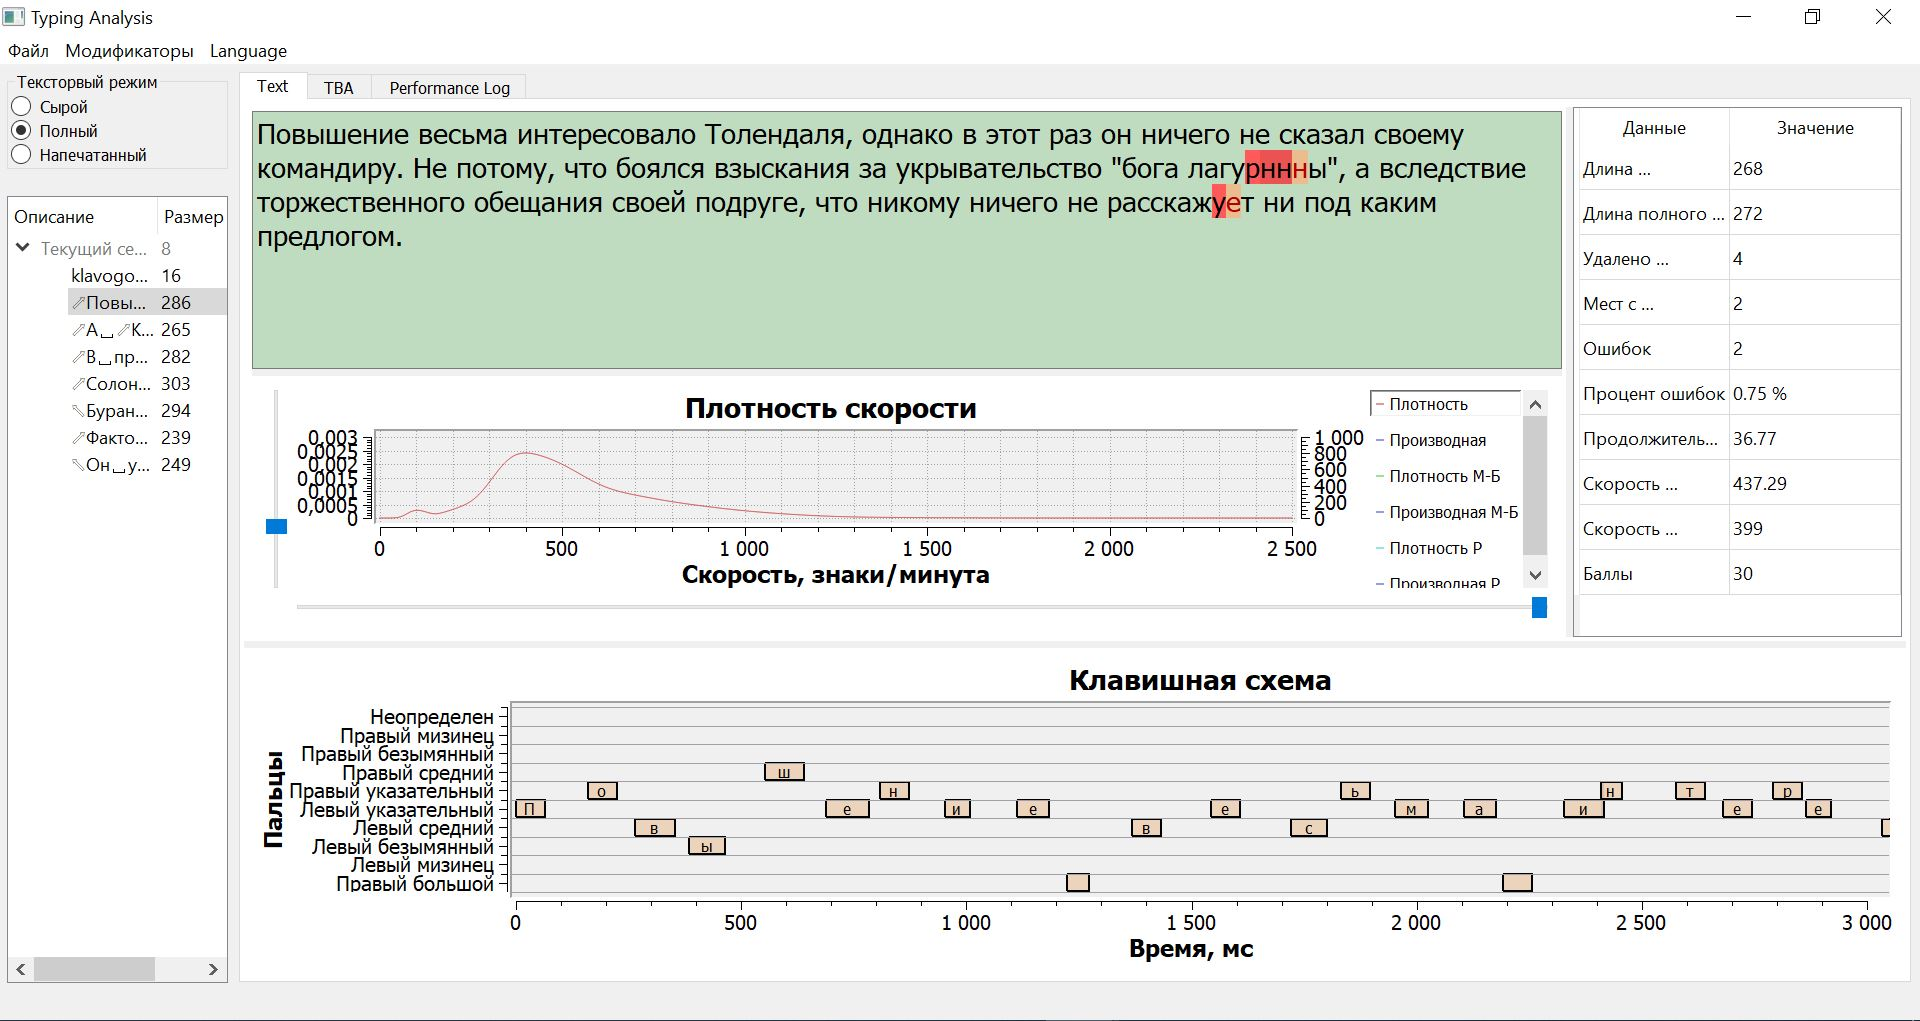
\includegraphics[scale=0.355]{Figures/appfull.JPG}
\end{center}
Давайте в общих чертах объясню, что здесь происходит.
Данная программа представляет из себя всего одно окно, которое вы видите на скриншоте выше.
Программа умеет находиться в двух режимах:
\begin{enumerate}
\item Режим перехвата клавиватуры.
В свернутом режиме, программа перехватывает весь ввод пользователя.

\item Режим анализа.
В развернутом режиме, программе не прослушивает клавиатуру, вместо этого она дает возможность посмотреть информацию о уже записанных данных, которые были перехвачены ранее.
\end{enumerate}
При переходе от прослушивающего состояния в состояние анализа все накопленные данные сгружаются в ядро программы.
Вся информация о наборе хранится в виде сессий.
Теперь опишем компоненты графического интерфейса.
\begin{enumerate}
\item
Слева вы видите список сессий, где отражено несколько первых клавиш нажатых в данную сессию, ее длина в количестве нажатых клавиш и какая сессия сейчас активна.
\begin{center}
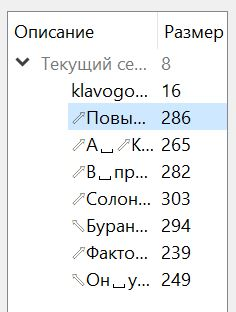
\includegraphics[scale=0.5]{Figures/SessView.JPG}
\end{center}

\item Над панелью для выбора сессий находится панель выбора режима для отображения перехваченного набора.
\begin{center}
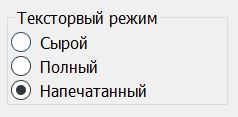
\includegraphics[scale=0.5]{Figures/textmodev.JPG}
\end{center}
Данный режим влияет на отображение сессии в текстовом окне описанном в пункте~\ref{item::TextView}.
Есть три режима
\begin{enumerate}
\item Сырой.
В нем отображаются все клавиши которые были нажаты независимо от того дают они символы или нет.

\item Полный.
В этом режиме отображаются только напечатанные символы включая все удаленные.
Удаленные символы подсвечиваются специальным образом.

\item Напечатанный.
В этом режиме отображается только конечный текст, который был напечатан без учета стертых символов.
\end{enumerate}

\item
\label{item::TextView}
Сверху по центру расположено текстовое окно предоставляющее информацию о перехваченной сессии.
\begin{center}
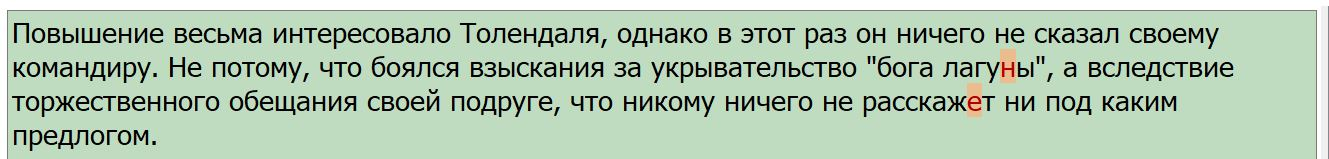
\includegraphics[scale=0.5]{Figures/TextView.JPG}
\end{center}

\item Ниже идет график плотности скорости.
\begin{center}
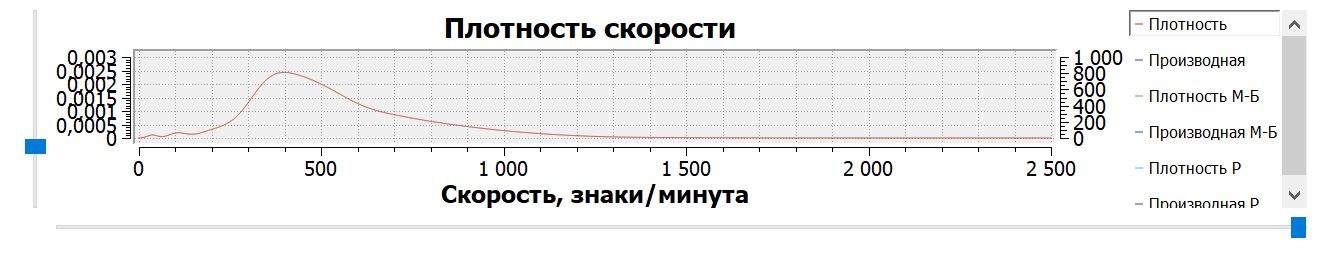
\includegraphics[scale=0.5]{Figures/plotView.JPG}
\end{center} 
Программа трактует скорость нажатия клавиши как случайную величину.
В данном окне приведена плотность распределения данной случайной величины.

\item Справа от текстового окна располагается окно статистики.
\begin{center}
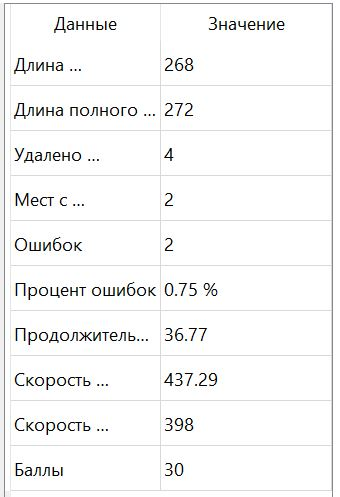
\includegraphics[scale=0.5]{Figures/StatView.JPG}
\end{center}
Самый интересный параметр -- предпоследний параметр -- это пик плотности распределения скорости.
Этот параметр хорошо характеризует скорость физических возможностей наборщика.

\item В самом низу находится клавишная схема, на которой отображается каким пальцем какая клавиша и в какой временной промежуток была нажата.
\begin{center}
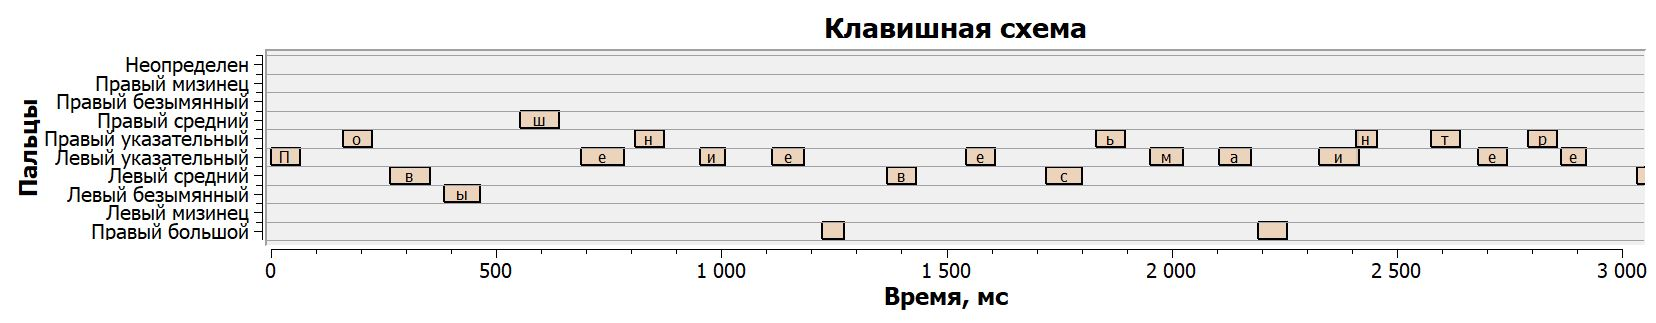
\includegraphics[scale=0.5]{Figures/DiagView.JPG}
\end{center}
\end{enumerate}
Тут стоит сказать, что от выбора текстового режима зависят: текстовое окно, график плотности и клавишная схема.
Вот пример как будет выглядеть та же самая сессия а напечатанном режиме.
\begin{center}
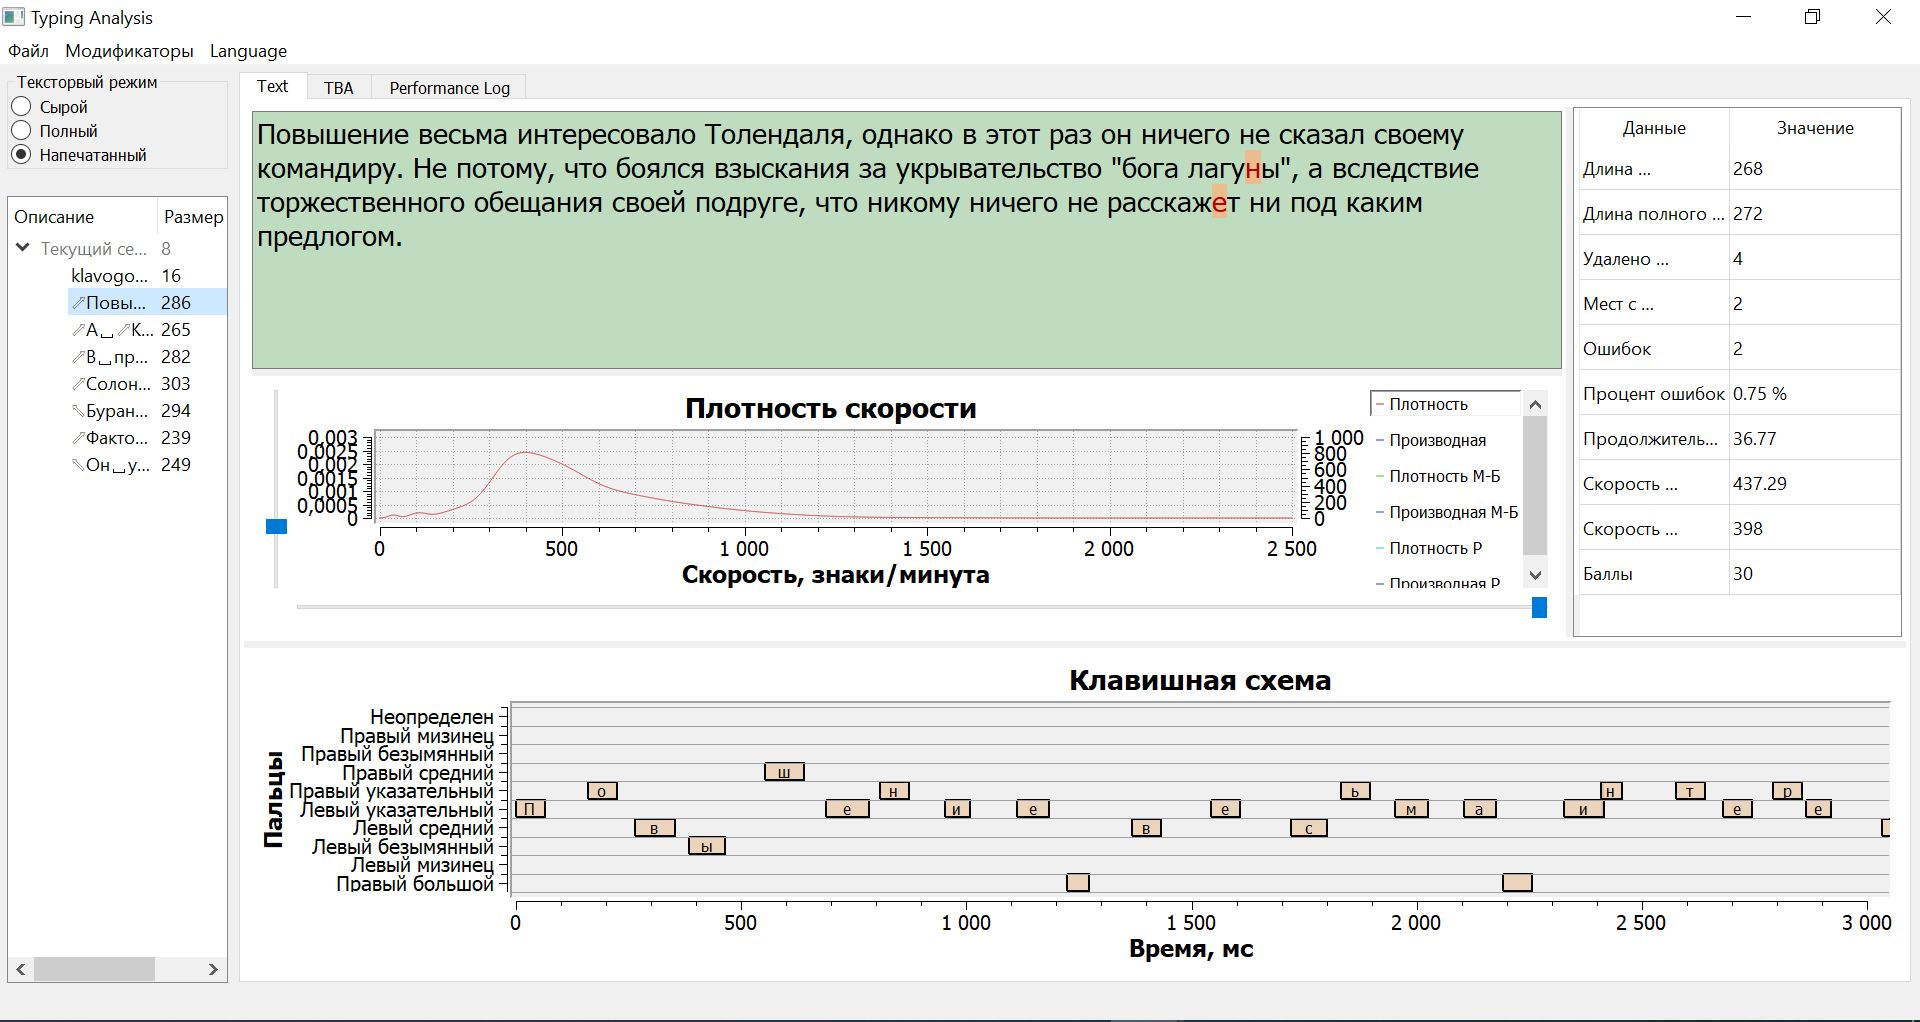
\includegraphics[scale=0.355]{Figures/appprint.JPG}
\end{center}
И в сыром режиме
\begin{center}
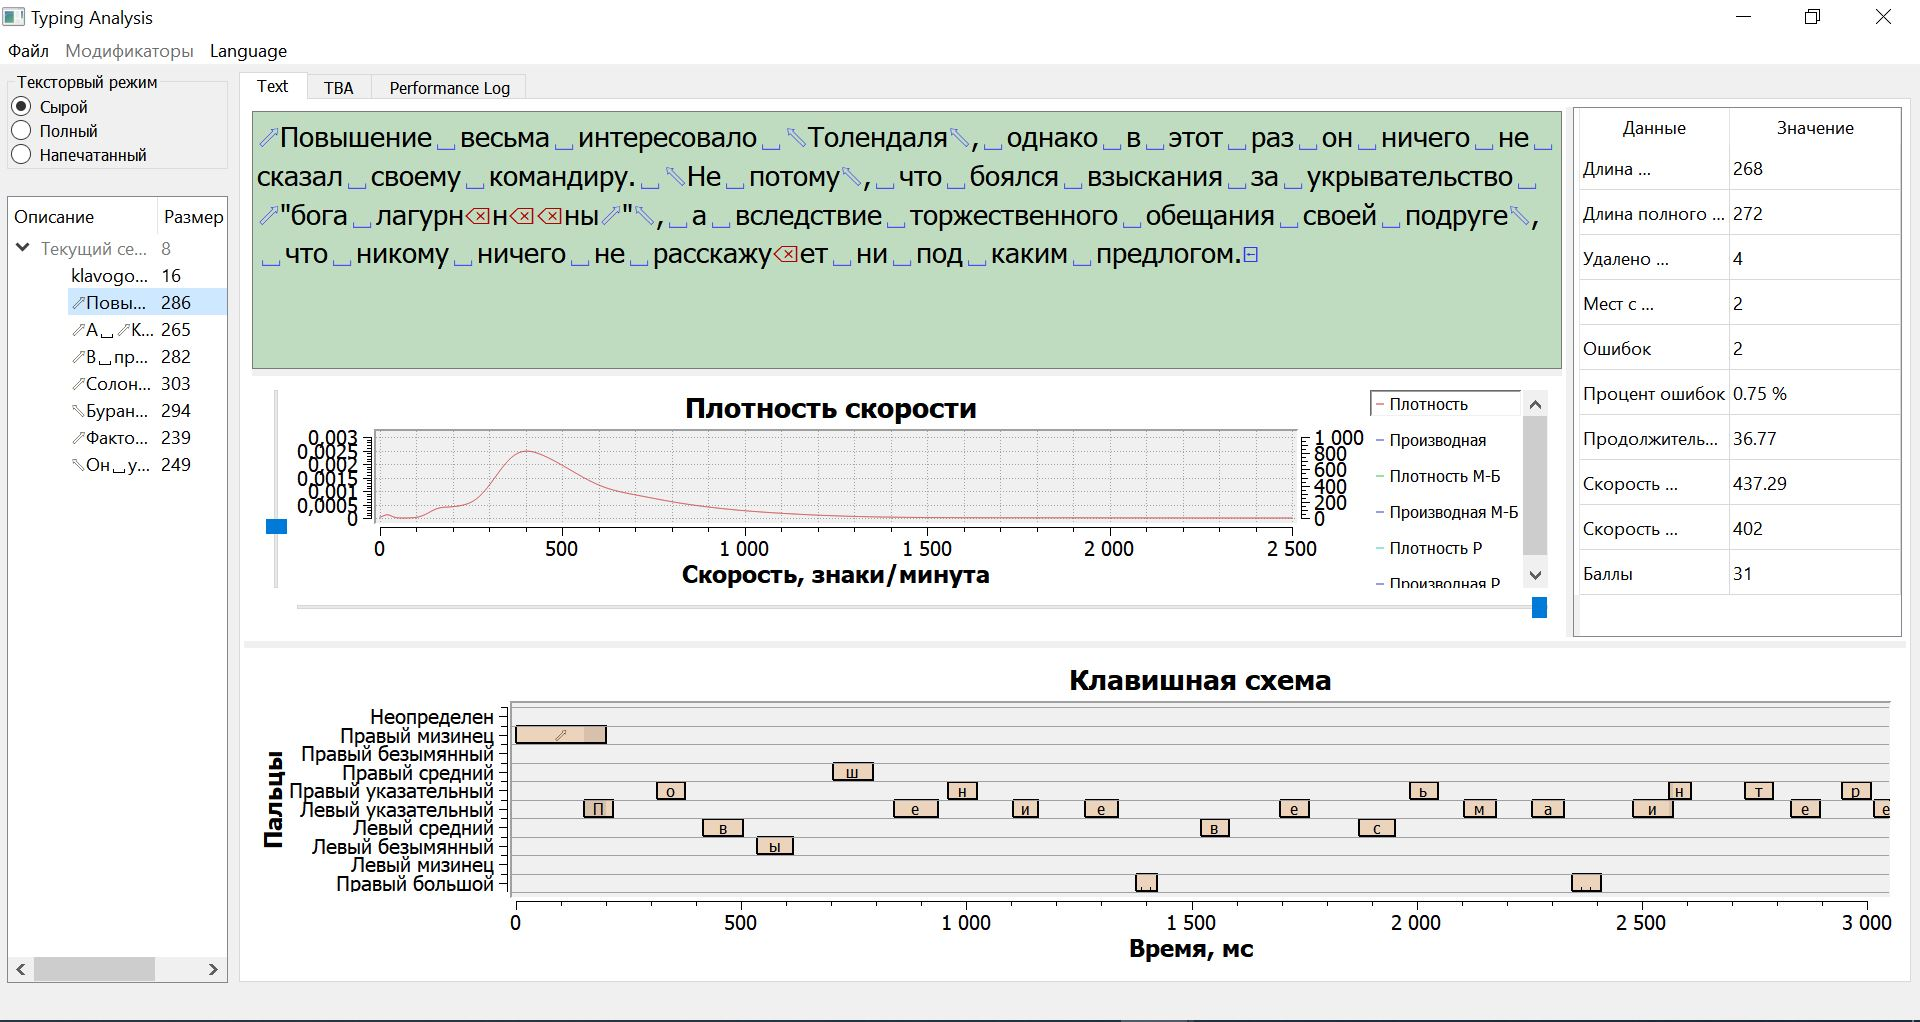
\includegraphics[scale=0.355]{Figures/appraw.JPG}
\end{center}
Видно, что в этом режиме появляются символы пробела, символы для backspace-а, для шифтов и прочие.

Давайте я продемонстрирую как выглядит часть приложения с точки зрения MVC.
\[
\resizebox{12cm}{!}{
\xymatrix@R=10pt{
  {}&{\parbox{1.5cm}{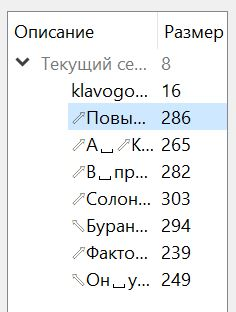
\includegraphics[scale=0.5]{Figures/SessView.JPG}}}\ar@{-->}[dl]&{}&{\parbox{1.5cm}{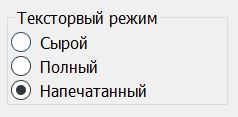
\includegraphics[scale=0.5]{Figures/textmodev.JPG}}}\ar@{-->}[dl]&{\parbox{3cm}{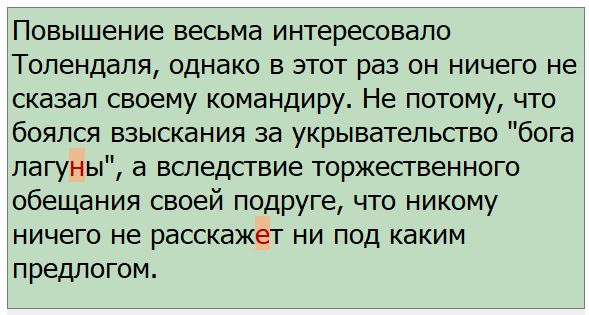
\includegraphics[scale=0.5]{Figures/TextView2.JPG}}}&{}&{\parbox{2cm}{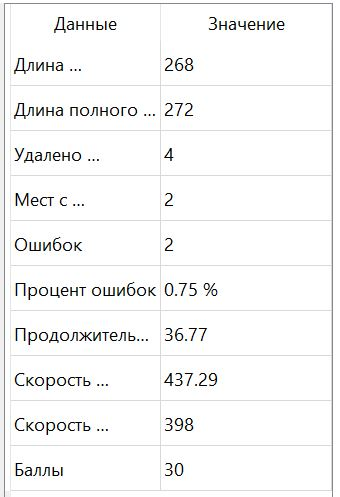
\includegraphics[scale=0.5]{Figures/StatView.JPG}}}&{}\\
  {\text{Ctrl}}\ar@{->>}[dr]&{}&{\text{Ctrl}}\ar@{->>}[dr]&{}&{}&{}&{}&{}\\
  {}\ar@{-->}[r]&{\text{Selector}}
  {\save
  [].[rrrrd]*+[F--]\frm{}
  \restore
  }
  \ar@{-->}[rr]\ar@{-->}[uu]&{}&{\text{Text}}\ar@{-->}[d]\ar@{-->}[r]\ar@{-->}[uu]\ar@{-->}[uur]
  &{\text{Math}}\ar@{-->}[r]\ar@{-->}[rddd]+(0,9)&{\text{Stat}}\ar@{-->}[uur]&{}&{}\\
  {}&{}&{\text{Layout}}\ar@{-->}[r]&{\text{Scheme}}\ar@{-->}[ddl]+(0,9)&{}&{\phantom{\text{Plot}}}&{}&{}\\
  {}&{}&{}&{}&{}&{}&{}\\
  {\parbox{1cm}{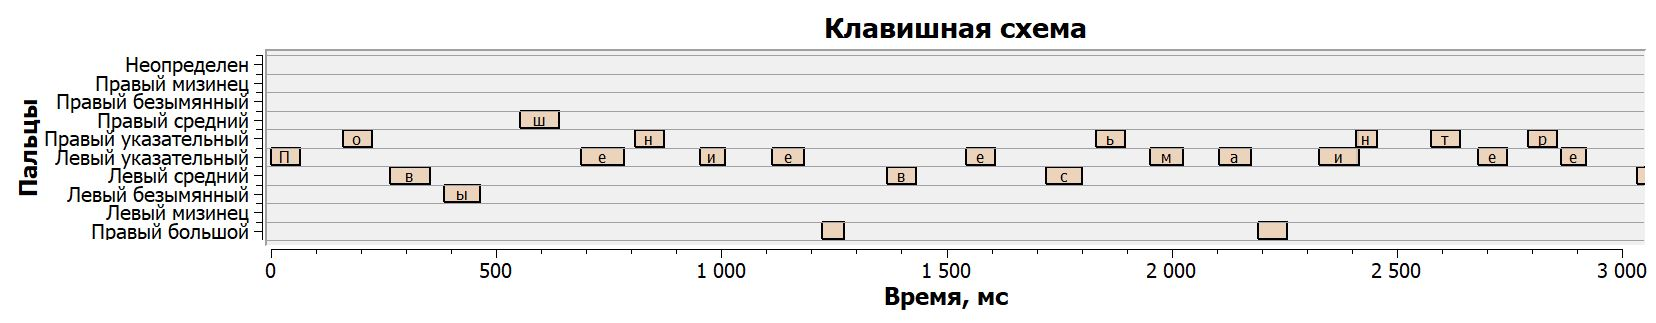
\includegraphics[scale=0.3]{Figures/DiagView.JPG}}}&{}&{}&{}&{\makebox[0.1cm][r]{\parbox{1cm}{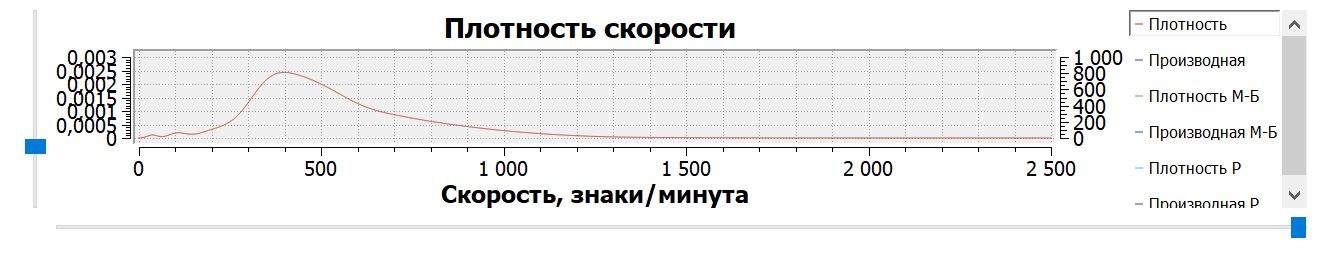
\includegraphics[scale=0.35]{Figures/plotView.JPG}}}}&{}&{}&{}\\
}
}
\]
Давайте я прокомментирую диаграмму выше.
\begin{itemize}
\item Часть выделенная пунктиром в центре -- это часть ядра программы.
Эта часть ничего не знает про графические библиотеки и способна работать без GUI.

\item Пунктирная стрелка слева ведет из другой части ядра, которая нам сейчас не очень важна, ибо в той части не используется MVC.

\item Ядро из себя представляет пайплайн, по которому данные проходят слева направо и после этого сообщаются пользователю через GUI.

\item Блок Selector выбирает текущую сессию для анализа.
Можно видеть MVC контур вокруг этого блока.
Selector является моделью в этом контуре.

\item Блок Text -- текстовый модуль.
Его задача хранить текущий режим и текст, который необходимо отобразить в текстовом окне.
Тут видно, что текстовое окно просто получает новые данные и через него нет возможности управления.
А выбор текстового режима -- это еще один MVC контур.

\item Блок Scheme -- модуль, который по распальцовке заданной пользователем и текущему режиму показывает диаграмму распределения нажатий по пальцам во времени.
Сама распальцовка хранится в модуле Layout и задается пользователем заранее.

\item Блок Math вычисляет плотность распределения скорости набора.
Он оповещает View отображающую плотность.

\item И в конце идет блок Stat, который является модулем статистики.
Он получает всю информацию из всех предыдущих модулей, вычисляет некую статистику и отображает ее в окне для статистики.
\end{itemize}
На этой диаграмме не отображены некоторые мелочи, как например выбор способа вычисления плотности распределения или локализация текста в элементах GUI.
Однако, я надеюсь, что эта схема хотя бы в общих чертах дает понять, как можно собирать подобное интерактивное приложение.
Так же отмечу, что все вызовы между компонентами блокирующие.
Это не очень хорошо, но это не сложно исправить имея value semantics для данных пересылаемых в observer паттерне.
Если вам интересна более детальная информация, то можно изучить \href{https://github.com/DimaTrushin/TypingAnalysis}{репозиторий} с проектом.
Там можно найти дизайн документацию с более подробным описанием происходящего.

\subsubsection{Пример 2 использования MVC}

Еще один пример, который я хочу привести -- это простая программа, которая показывает пользователю поле с двумя фишками и эти фишки можно двигать только на соседние клетки по вертикали и горизонтали.
Больше ничего делать нельзя.
Как обычно приведу скриншот в самом начале.
\begin{center}
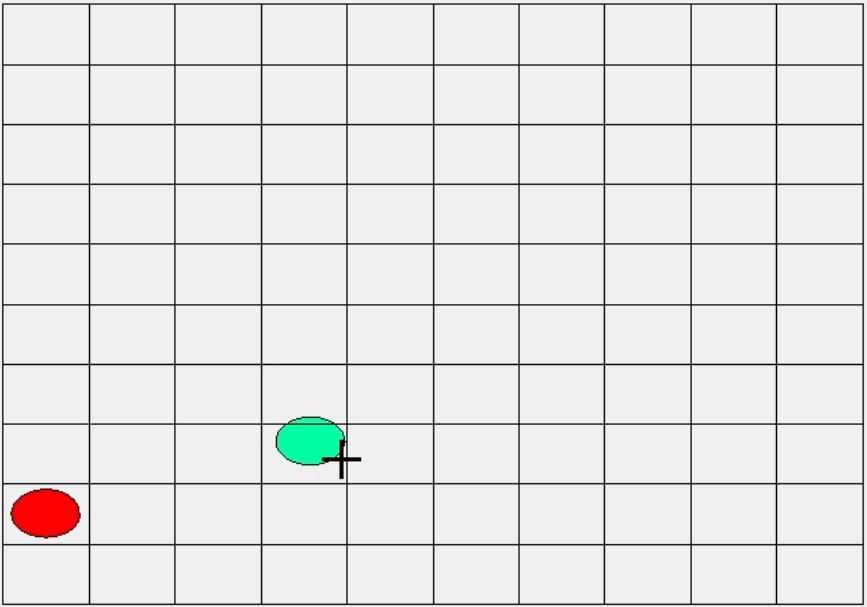
\includegraphics[scale=0.6]{Figures/Game1.JPG}
\end{center}
Ожидаемое поведение программы такое.
Вы можете подцепить курсором фишку и перемещать ее держа зажатой левую клавишу мыши.
В момент перемещения захваченной фишки проигрывается настраиваемая анимация.
При отпускании фишки программа пытается поставить ее на указанное поле.
Если шаг сделать не возможно, то фишка возвращается в исходное состояние, откуда она была захвачена.

Важно понять, что в данном случае у нас не одна, а две модели.
\begin{enumerate}
\item Первая модель знает размер поля, расположение на нем фишек и правила, по которым фишкам можно ходить.
Эта модель оперирует целыми координатами фишек, обозначающие столбец и строку, где находится фишка.
Она ничего не знает про отображение поля, про фишки, про цвета, анимацию и прочее.
Это как бы <<внутренняя логика игры>>.

\item Вторая модель -- это геометрическая модель.
Дело в том, что в первой модели не достаточно информации для того, чтобы ее отрисовать.
Например не ясно каким цветом и как рисовать поле, какие должны быть размеры клеток, какие размеры, цвет и форма фишек.
Кроме того, при захвате фишки курсором она может находиться в состоянии, не имеющем смысла для модели игры.
Потому для отображения геометрии мы используем вторую модель.
\end{enumerate}
Схематически устройство программы выглядит так.
\[
\xymatrix{
  {\verb"model"}\ar@{-->}[rr]
  	{
	\save
   [].[]*+[F-:<3pt>]\frm{}
   \restore
	}
	{
	\save
   []+(-10,6).[drrrr]*+(3,0)++[F-:<3pt>]\frm{}
   \restore
	}
  &{}&{\verb"gmodel"}\ar@{-->}[rr]\ar@{-->}[dl]
      	{
	\save
   [].[]*+[F-:<3pt>]\frm{}
   \restore
	}
  &{}&{\verb"view"}\ar@{-->}[dl]
      	{
	\save
   [].[]*+[F-:<3pt>]\frm{}
   \restore
	}
  \\
  {}&{\verb"ctrl"}\ar@{->>}[lu]
      	{
	\save
   [].[]*+[F-]\frm{}
   \restore
	}
  &{}&{\verb"gctrl"}\ar@{->>}[lu]
      	{
	\save
   [].[]*+[F-]\frm{}
   \restore
	}
  &{}\\
}
\]
Давайте опишем все ее компоненты.
\begin{itemize}
\item model.
Это первая модель которая отвечает за
\begin{enumerate}
\item состояние поля

\item позиции фишек на поле

\item правила как фишки могут ходить
\end{enumerate}

\item gmodel.
Это вторая геометрическая модель.
Она отвечает за:
\begin{enumerate}
\item Система координат на плоскости.

\item Изображение поля

\item Изображение фишек

\item Анимация фишек при захвате

\item Информация какая фишка сейчас выбрана и является активной
\end{enumerate}

\item view.
Это View компонент.
Он не содержит состояния и лишь отрисовывает текущее состояние gmodel.

\item gctrl.
Контроллер управления геометрической моделью.
Позволяет
\begin{enumerate}
\item Захватить фишку при зажатии левой клавиши мыши.
При этом данная фишка становится активной в геометрической модели.

\item Двигать гоеметрическое представление активной фишки.

\item Отпустить захваченную фишку.
При этом фишка перестает быть активной.
\end{enumerate}

\item ctrl.
Это контроллер, который идет от геометрической модели к обычной модели.
Когда пользователь перетащил изображение фишки куда-то, гометерическая модель должна попросить обычную модель попытаться сделать предлагаемый ход.
И это управление делается через данный контроллер.
\end{itemize}
Давайте скажу пару слов по поводу поведения в такой схеме.
Если пользователь отпускает фишку в геометрической модели, то она оповещает View, чтобы та показала, где фишка остановилась.
Но сразу после этого оповещается контроллер модели, который дергает у модели метод, пытающийся сходить фишкой так, как просит геометрическая модель.
Далее модель либо ходит фишкой как сказано, либо отвергает действие.
Но в любом случае после этого она оповещает всех, кто на нее подписан.
В данном случае она оповещает геометрическую модель.
Которая при получении новых данных начинает отражать состояние модели, где фишка либо перемещена на новое поле, либо вернулась назад.
После чего оповещается View, чтобы отрисовать состояние геометрической модели.
Таким образом мы как бы оповещаем View дважды, но это нас устраивает, потому что одно оповещение -- это точка сброса фишки, а другое оповещение -- это исправленное состояние геометрической модели после попытки сделать ход.

\paragraph{Архитектура приложения}

Визуально архитектуру приложения можно представлять себе так.
\[
\xymatrix@R=15pt{
  {\verb"App"}
    {
	\save
   [].[d]*+[F-:<3pt>]\frm{}
   \restore
	}
  &{}&{}&{}\\
  {\verb"u\_ptr"}\ar[r]+(-13,0)&{}
    {
	\save
   []+(-13,4).[dddddrr]*+(8,0)+[F-:<3pt>]\frm{}
   \restore
	}
  &{\verb"AppImpl"}&{}\\
  {}&{\verb"AppKernel"}
  {
	\save
   [].[ddd]*+[F-:<3pt>]\frm{}
   \restore
	}
  &{}&{\verb"AppGui"}
  {
	\save
   [].[d]*+[F-:<3pt>]\frm{}
   \restore
	}
  \\
  {}&{\verb"model"}\ar@{-->}@<3ex>@/^/[dd]&{}&{\verb"view"}\ar@{-->}@(d,r)[dddl]\\
  {}&{\verb"ctrl"}\ar@{->>}[u]&{}&{}\\
  {}
  &{\verb"gmodel"}\ar@{-->}[u]\ar@{-->}[rruu]&{}&{}\\
  {}&{}&{\verb"gctrl"}\ar@{->>}@(l,d)[lu]
  &{}\\
}
\]
Давайте про комментируем, что тут происходит.
\begin{itemize}
\item Объект \verb"App" -- это главный объект нашего приложения.
Для него используется Pimpl (см. раздел~\ref{section::Pimpl}), чтобы разгрузить стек вызовов.

\item Вся имплементация спрятана внутрь \verb"AppImpl".
При этом для улучшения локальности мы выделяем в имплементации два раздела посвященных ядру и GUI.

\item \verb"AppKernel" -- кусок \verb"AppImpl", в котором находятся компоненты ядра.
Технически это базовый класс \verb"AppImple".
В данном случае наследование используется как композиция.
Тут живут model, gmodel и ctrl.

\item \verb"AppGui" -- кусок \verb"AppImpl", в котором находятся все GUI компоненты.
В данном случае это просто view компонента.

\item Контроллер gctrl должен соединять GUI и ядро.
Потому он располагается в \verb"AppImpl" непосредственно.
\end{itemize}
В коде это выглядит так.
\begin{center}
\begin{tabular}{c}
\begin{tabular}{cc}
{
\begin{minipage}[\baselineskip]{8cm}
\begin{cppcode}[numbers = none]
class AppKernel {
  AppKernel()
   : ctrl_(&model_) {
    model_.subscribe(gmodel.port());
    gmodel_.subscribe(ctrl_.port());
  }
protected:
  Model model_;
  GModel gmodel_;
  Ctrl ctrl_;
};
\end{cppcode}
\end{minipage}
}
&
{
\begin{minipage}[\baselineskip]{8cm}
\begin{cppcode}[numbers = none]
class MainWindow {
public:
  View* view();
private:
  View view_;
};

class AppGui {
protected:
  MainWindow window_;
};
\end{cppcode}
\end{minipage}
}
\end{tabular}
\\
\begin{minipage}[\baselineskip]{8cm}
\begin{cppcode}
class AppImpl : AppKernel, AppGui {
public:
  AppImpl() : gctrl_(&gmodel_) {
    gmodel_.subscribe(view()->port());
    view()->subscribe(gctrl_.port());
  }
protected:
  GCtrl gctrl_;
};
\end{cppcode}
\end{minipage}
\end{tabular}
\end{center}
Структура здесь в точности такая как описано выше.
Надо лишь прокомментировать как работают конструкторы.
\begin{enumerate}
\item \verb"AppKernel" в своем конструкторе соединяет компоненты ядра.
Причем в этом дизайне у меня контроллер приваривается к модели в своем конструкторе.
А observable/observer порты надо соединить в теле конструктора.

\item \verb"AppGui" содержит одну компоненту -- основное окно, в котором располагается \verb"view" объект.
Основное окно собирается из Qt кода.

\item Далее все компоненты соединяются в \verb"AppImpl".
С помощью наследования я включаю ядро и GUI часть в имплементацию.
А потом в конструкторе делаю все оставшиеся соединения.
\end{enumerate}

Код приложения можно найти в \href{https://github.com/DimaTrushin/InteractiveGUI}{репозитории}.

\paragraph{Другая вариация приложения}

У этого приложения можно легко сделать вариацию с любым количеством view и геометрических моделей.
Очень полезно понимать, что будет происходить при разных вариациях их соединения.
Начну как обычно со скриншота.
\begin{center}
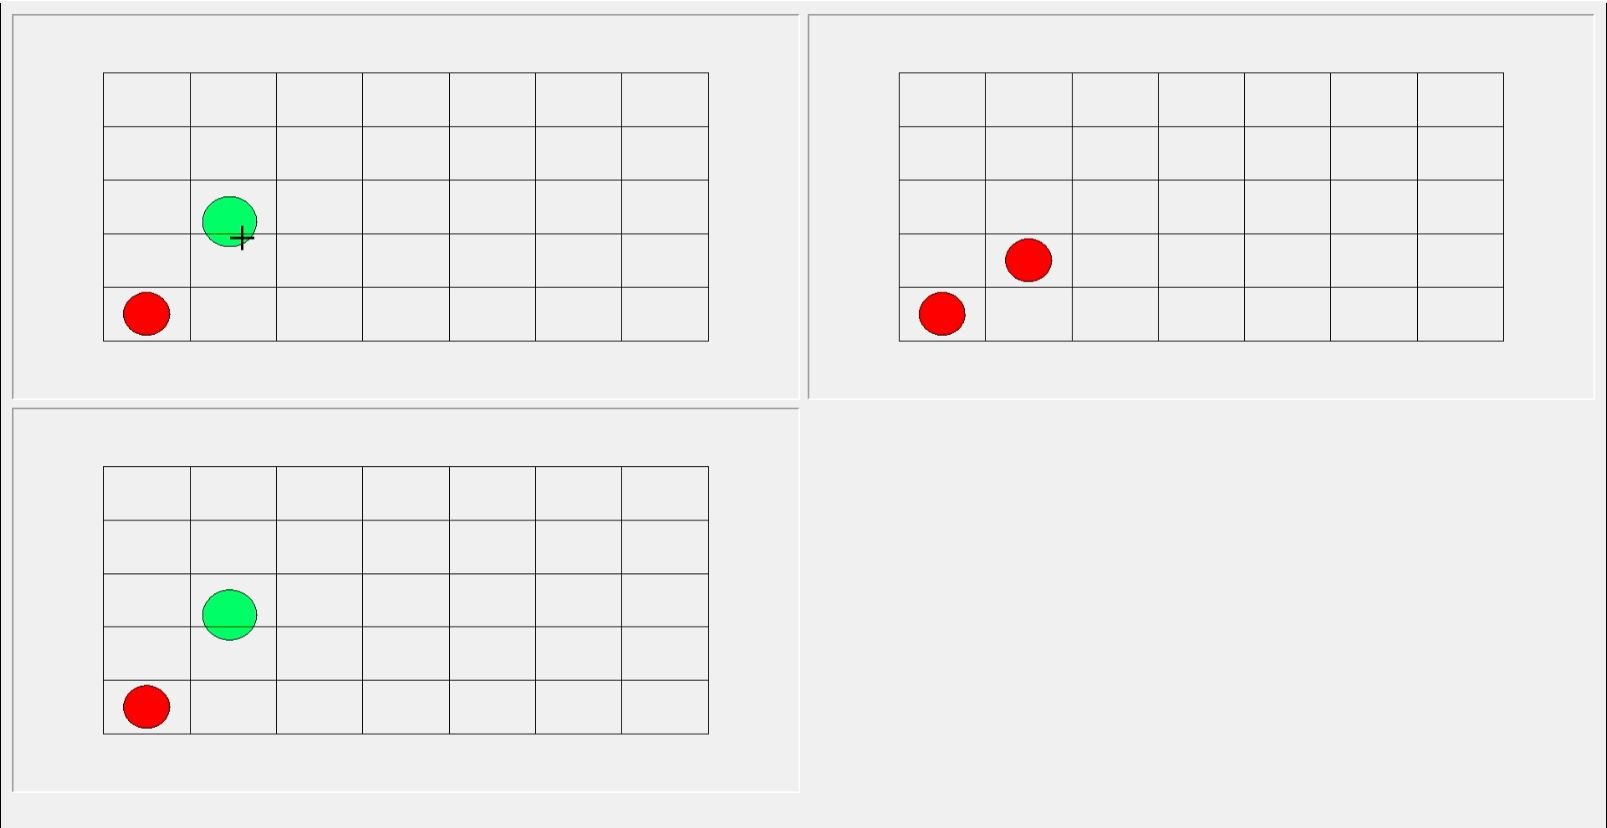
\includegraphics[scale=0.4]{Figures/Game2.JPG}
\end{center}
В этом случае поля слева синхронизированы на уровне геометрической модели.
А поле справа имеет свою геометрическую модель.
Нижнее поле без контроллера, через него управлять нельзя.
Если захватить фишку на левом поле и двигать захваченную фишку по полю, то ее движение будет видно только на двух левых полях.
Но если фишку отпустить на клетку допустимого хода, то обновятся все три поля разом.
Аналогично, если мы захватим фишку на правом поле, то ее перемещение будет видно только на нем, но когда мы сделаем ход, то обновятся все три поля.

Вот схема соединения объектов.
\[
\xymatrix@R=15pt{
  {}
     {\save
  []+(-10,5).[ddddddrrrr]*+(4,0)+[F-:<3pt>]\frm{}
  \restore
  }
  &{}&{\verb"AppImpl"}&{}&{}\\
 {}
   {\save
  []+(-8,5).[dddddrr]*+(7,0)+[F-:<3pt>]\frm{}
  \restore
  }
 &{\verb"AppKernel"}&{}&{}&{\verb"AppGui"}
    {\save
  []+(-8,5).[ddddd]*+(1,0)+[F-:<3pt>]\frm{}
  \restore
  }
 \\
  {}
  &{\verb"ctrl1"}\ar@{->>}[ldd]
    {\save
  [].[]*[F-:<3pt>]\frm{}
  \restore
  }
  &{}&{\verb"gctrl1"}\ar@{->>}[ld]
    {\save
  [].[]*[F-:<3pt>]\frm{}
  \restore
  }
  &{\verb"view1"}
  \ar@{-->}@/_/[l]
    {\save
  [].[]*[F-:<3pt>]\frm{}
  \restore
  }
  \\
  {}&{}&{\verb"gmodel1"}
  \ar@{-->}[lu]
  \ar@{-->}@/_/[urr]
  \ar@{-->}@/^/[drr]
    {\save
  [].[]*[F-:<3pt>]\frm{}
  \restore
  }
  &{}&{}\\
  {\verb"model"}
  \ar@{-->}[rru]
  \ar@{-->}[rrd]
  {\save
  [].[]*[F-:<3pt>]\frm{}
  \restore
  }
  &{}&{}&{}
  &{\verb"view2"}
    {\save
  [].[]*[F-:<3pt>]\frm{}
  \restore
  }
  \\
  {}&{}&{\verb"gmodel2"}
    \ar@{-->}[ld]
  \ar@{-->}@/^/[drr]
    {\save
  [].[]*[F-:<3pt>]\frm{}
  \restore
  }
  &{}&{}\\
  {}&{\verb"ctrl2"}\ar@{->>}[luu]
    {\save
  [].[]*[F-:<3pt>]\frm{}
  \restore
  }
  &{}&{\verb"gctrl2"}\ar@{->>}[lu]
    {\save
  [].[]*[F-:<3pt>]\frm{}
  \restore}&{\verb"view3"}
    \ar@{-->}@/^/[l]
  {\save
  [].[]*[F-:<3pt>]\frm{}
  \restore
  }
  \\
}
\]
Эта диаграмма напрямую транслируется в код, потому я не буду его тут приводить.

\paragraph{Точка входа в программу}

Данное приложение собиралось в экосистеме Qt с использованием не блокирующего Observer Pattern.
Вот как выглядит функция \verb"main"
\begin{cppcode}
#include "Application.h"
#include "Except.h"
#include "QRunTime.h"

int main(int argc, char* argv[]) {
  QApp::QRunTime runtime(argc, argv);
  try {
    QApp::Application app;
    runtime.exec();
  } catch (...) {
    QApp::Except::react();
  }
  return 0;
}
\end{cppcode}
Сделаем несколько замечаний:
\begin{enumerate}
\item \verb"QRunTime" -- это наша надстройка над Qt runtime-ом, которая позволяет общению неблокирующего observer-а.
Этот объект в начале функции \verb"main" инициализирует всю экосистему и запускает event loop вызовом функции \verb"exec".

\item \verb"Application" -- это класс нашего приложения.
Он является пассивным объектом в Qt экосистеме.
Он ничего не выполняет сам, он и его компоненты лишь реагируют на Qt сообщения и посылают свои.

\item Обратите внимание, что функция \verb"main" ничего не делает сама.
Она всю работу делегирует другим объектам.
Даже обработку исключений.

\item Одна из задач функции \verb"main" -- не допустить утекания исключений в OS.
Это нужно для того, чтобы отличить ошибки которые возникли в программе из-за самой программы от ошибок, которые возникли в программе из-за операционной системы.
\end{enumerate}
При этом обработка исключений выглядит так
\begin{cppcode}
#include "Except.h"
#include <QDebug>
#include <exception>

namespace QApp {
namespace Except {
void react() noexcept {
  try {
    throw;
  } catch (std::exception& e) {
    qDebug() << "Exception: " << e.what();
  } catch (...) {
    qDebug() << "Enknown Exception!";
  }
}
} // namespace Except
} // namespace QApp
\end{cppcode}
Функция react будет вызвана внутри блока \verb"catch", а значит в этот момент есть активное исключение.
Чтобы его еще раз поймать, мы просто внутри \verb"try" блока делаем \verb"throw" без аргументов.
И уже после в разных видах \verb"catch" ловим исключения и реагируем на них.
Все это замечательно за одним большим исключением: Qt не разрешает бросать исключения в event loop.
Это связано с тем, что Qt изначально не планировал поддерживать исключения.
Как мы понимаем сейчас это большая ошибка.
Все новые компоненты Qt пишутся в парадигме exception safe.
Однако, все ключевые компоненты ядра все еще не поддерживают бросание исключений и это большой геморрой.

\subsubsection{MVVM}

Теперь я хочу поговорить о паттерне Model/View/View-Model.
Прежде чем к нему переходить, давайте вспомним наш пример с Widget-ом, который имел внутреннее состояние.
\[
\xymatrix{
  {}&{}&{}&{
  \textbf{Widget}
  }&{}\\
  {}&{}&{
  \phantom{\text{V}}\text{M}
  }
  \ar@{-->}@<0.6ex>[rr]
  {\save
  [].[rrd]*++[F-]\frm{}
  \restore
  }
  &{}&{
  V
  }
  {\save
  [].[d]*++\frm{}
  \restore
  }
  \ar@{-->}[dl]
  \\
  {
  \text{Model}
  }
  \ar@{-->}@(u,l)[urr]
  &{}&{\phantom{\text{Model}}}
  \ar@{-->}@(d,r)[dl]
  &{
  \text{C}
  }
  \ar@{->>}[ul]
  &{\phantom{\text{C}}}
  \\
  {}&{
 \text{Ctrl}
  }
  \ar@{->>}@(l,d)[ul]
  &{}&{}&{}\\
}
\]
Теперь я хочу помодифицировать чуть-чуть эту конструкцию.
Так как внутри Widget-а у нас view оповещает только один контроллер, то в самом начале их можно слить в одну сущность.
\[
\xymatrix{
  {}&{}&{}&{\textbf{Widget}}&{}\\
  {}&{}&{\phantom{\text{V}}\text{M}}\ar@{-->}@(d,r)[ddl]\ar@{-->}@<0.6ex>[rr]
  {\save
  [].[rr]*++[F-]\frm{}
  \restore
  }
  &{}&{\text{V}}\ar@{->>}@<0.6ex>[ll]\\
  {\text{Model}}\ar@{-->}@(u,l)[urr]&{}&{\phantom{\text{Model}}}&{}&{\phantom{\text{C}}}\\
  {}&{\text{Ctrl}}\ar@{->>}@(l,d)[ul]&{}&{}&{}\\
}
\]
Теперь можно вынуть внутреннюю модель наружу, оставив общение с внутренностями Widget-а через фиксированный интерфейс.
\[
\xymatrix{
  {}&{}&{}&{\textbf{Widget}}&{}\\
  {}&{}&{\text{VM}}\ar@{-->}@<0.6ex>[rr]
  {\save
  [].[rr]*++[F-]\frm{}
  \restore
  }
  &{}&{\text{V}}\ar@{->>}@<0.6ex>[ll]\\
  {\text{Model}}\ar@{-->}[rr]+(-2,0)&{}&{\phantom{\text{od}}\text{M}\phantom{\text{el}}}\ar@{->}[u]\ar@{-->}@(d,r)[dl]&{}&{}\\
  {}&{\text{Ctrl}}\ar@{->>}@(l,d)[ul]&{}&{}&{}\\
}
\]
Ну а теперь просто нет необходимости во второй модели.
И мы получаем.
\[
\xymatrix{
  {}&{}&{}&{\textbf{Widget}}&{}\\
  {}&{}&{\text{VM}}\ar@{-->}@<0.6ex>[rr]
  {\save
  [].[rr]*++[F-]\frm{}
  \restore
  }
  &{}&{\text{V}}\ar@{->>}@<0.6ex>[ll]\\
  {\phantom{\text{Model}}}&{}&{\text{Model}}\ar@{->}[u]&{}&{}\\
  {}&{\phantom{\text{Ctrl}}}&{}&{}&{}\\
}
\]
Давайте я прокомментирую, что тут произошло.
Для того, чтобы сделать view stateless нам нужно как-то внутри view получать данные из модели.
Понятно, что их можно получать по observer паттерну, но проблема в том, в каком формате они должны быть.
Так вот формат данных для view -- это первое что надо фиксировать.
Кроме того, если мы хотим управлять произвольной моделью не зная, как она устроена, то нам нужна вспомогательная прослойка, которая на картинке изображена как VM.
Это по сути интерфейс для общения с моделью.
Это не обязательно интерфейс в смысле наследования с виртуальными функциями.
Это может быть стирающий указатель (см. раздел~\ref{section::RefErasure}).
В такой модели интерфейс View Model соединяется напрямую с View, потому что ей больше не с кем соединяться.
А Model подключается к View Model уже внешне.
Такой подход называется Model/View/View-Model.
Важно понимать, что он ни в коем случае не отменяет MVC.
